\section{Experimental setup}
\subsection{The OPAL detector}
\label{sec:experimentalsetup}
Modern experimental physics use large circular colliders in order to approach energies necessary for the
specific resonances. In particular, the Large Electron-Positron Collider (\textbf{LEP}), whose data we are using, was one
of the largest accelerator ever constructed with a circumference of 27 kilometres. Electron and positron packets are brought
to energies from $\sqrt{s} = 88$ GeV up to $\sqrt{s} = 94$ GeV in order to examine the gauge bosons of the weak interaction. 
The Experiments \textbf{OPAL}, \textbf{DELPHI}, \textbf{ALEPH} and \textbf{L3} were conducted to measure the electron-positron
collisions. However, we will only look at \textbf{OPAL}. 
The abbreviation stands for  "\textbf{O}mni \textbf{P}urpose \textbf{A}pparatus at \textbf{L}EP", stating that the 
measurements can be used to tackle different issues. The experiment started in
1989 and data was taken until the year 2000. The collaboration consisted of some 200 physicists from 34 institutes.
The main ingredients of the experiment are the following: 
\begin{itemize}
    \item \emph{Tracking Detectors}: The tracking system is built up with increasing radius, consisting of 
        a \textit{silicon microvertex detector}, a \textit{vertex detector}, 
        a \textit{jet chamber}, and \textit{z-chambers} 
        (see figure~\ref{fig:opal1} for a detailed schematic representation). In general, these tracking detectors
    are triggered by the ionization when charged particles are passing by. 
    The \textit{jet chamber} helps identifying particles, since their so-called 
\textit{ionization energy loss} $\frac{dE}{dx}$ depends on momentum and type ($\rightarrow$ charge). For
    more details about the single chambers please refer to \cite{CERN_OPAL}.
\item \emph{Calorimeter}: Calorimeters exploit the principle of particle-matter interaction and are thus
    composed of dense material. For the different fermion types there are different calorimeters: Electromagnetic calorimeter
    are made of lead-glass blocks and measure the energy of electrons/positrons and photons. Hadron calorimeter are located
    farther away from the center and are made of iron with a width of about one meter. 
\item \emph{Muon detectors}: Since muons are most likely not absorbed by the already mentioned calorimeters, it is necessary 
        to use additional muon chambers to track them down. Muons are least ionizing particles with very little energy
        loss in solid materials. The muon chambers consist of a mixture of argon, methane, carbon dioxide and work analogously to
        the tracking detectors. 
\end{itemize}
As it should be clear by now, the magnitude of the detector is due to the need to measure the particle momenta and energies
precisely enough, since this is the only possibility to distinguish them from each other. 
Due to their high energies, some showers need up to one meter depth of iron to be absorbed. 
\begin{figure}[htpb]
    \centering
    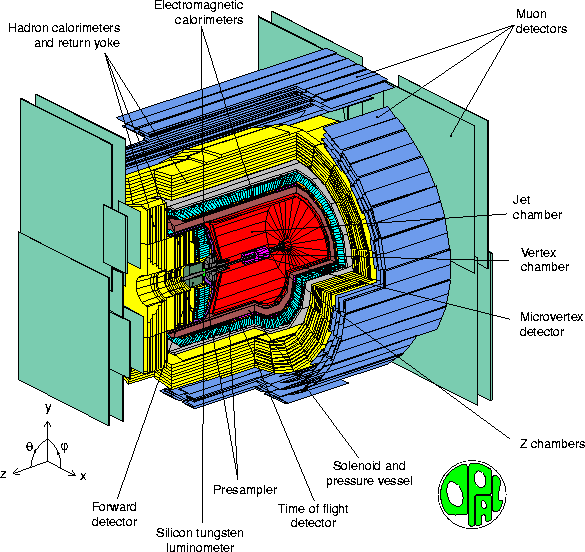
\includegraphics[width=1.0\linewidth]{figures/opal}
    \caption{The image shows a cut-away view of the \textbf{OPAL} detector. The layered structure of the
    different chambers, which encase the central beam pipe, can be distinguished clearly. The beams are essentially
    prepared to be mono-energetic. They collide at the center of the detector (near the Microvertex detector).
    Taken from \cite{CERN_OPAL}.}
    \label{fig:opal1}
\end{figure}

\begin{figure}[htpb]
    \centering
    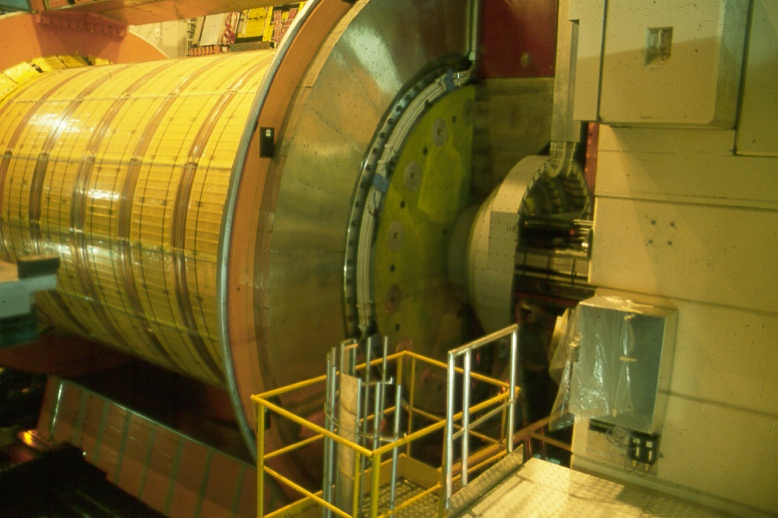
\includegraphics[width=1.0\linewidth]{figures/opal_photo}
    \caption{Photography of the early installation of the \textbf{OPAL} detector, spring 1988. 
        The experiment's extents were $12m \times 12m \times 12m$. 
        It was dismantled in 2001 due to the construction of the LHC. On the right one can see the outer structure of the detector, 
        for more technical details refer to figure~\ref{fig:opal1}. 
        From \cite{CERN_OPAL}.}
    \label{fig:opal_photo}
\end{figure}

\subsection{Background}
\label{sub:background}
The constraints on the detectors involved in the experiment govern the purity of our signal. Here we
discuss possible background effects and their order of magnitude~\cite{ver}.
\begin{itemize}
    \item \textit{Electronic noise:} Working with electronic devices we can never eliminate their delimiting influence. 
        Their signal
        can superimpose the true signal and give rise to misleading interpretations. This is why photons below 1 GeV cannot
        be resolved.
    \item \textit{The construction and geometry of the detector} is not continuous, there is always the possibility to hit a gap.
        One method to eliminate this effect is to reconstruct all trajectories and analyze the position of this gaps very
        carefully in order to track these particles as well.
    \item \textit{Efficiency of calorimeter} is not 100\%, so we need to extrapolate already tracked particles to make
    the corresponding losses visible.
\item \textit{Beam-gas} events are scattered electrons or positrons of the beam interacting with the rest gas in the vacuum
    tube. These events can be identified by looking at their interaction center,
    which lies necessarily outside the detector center. Furthermore, most particles will go into one direction.  
\end{itemize}



